\begin{figure}[H]
	\centering
	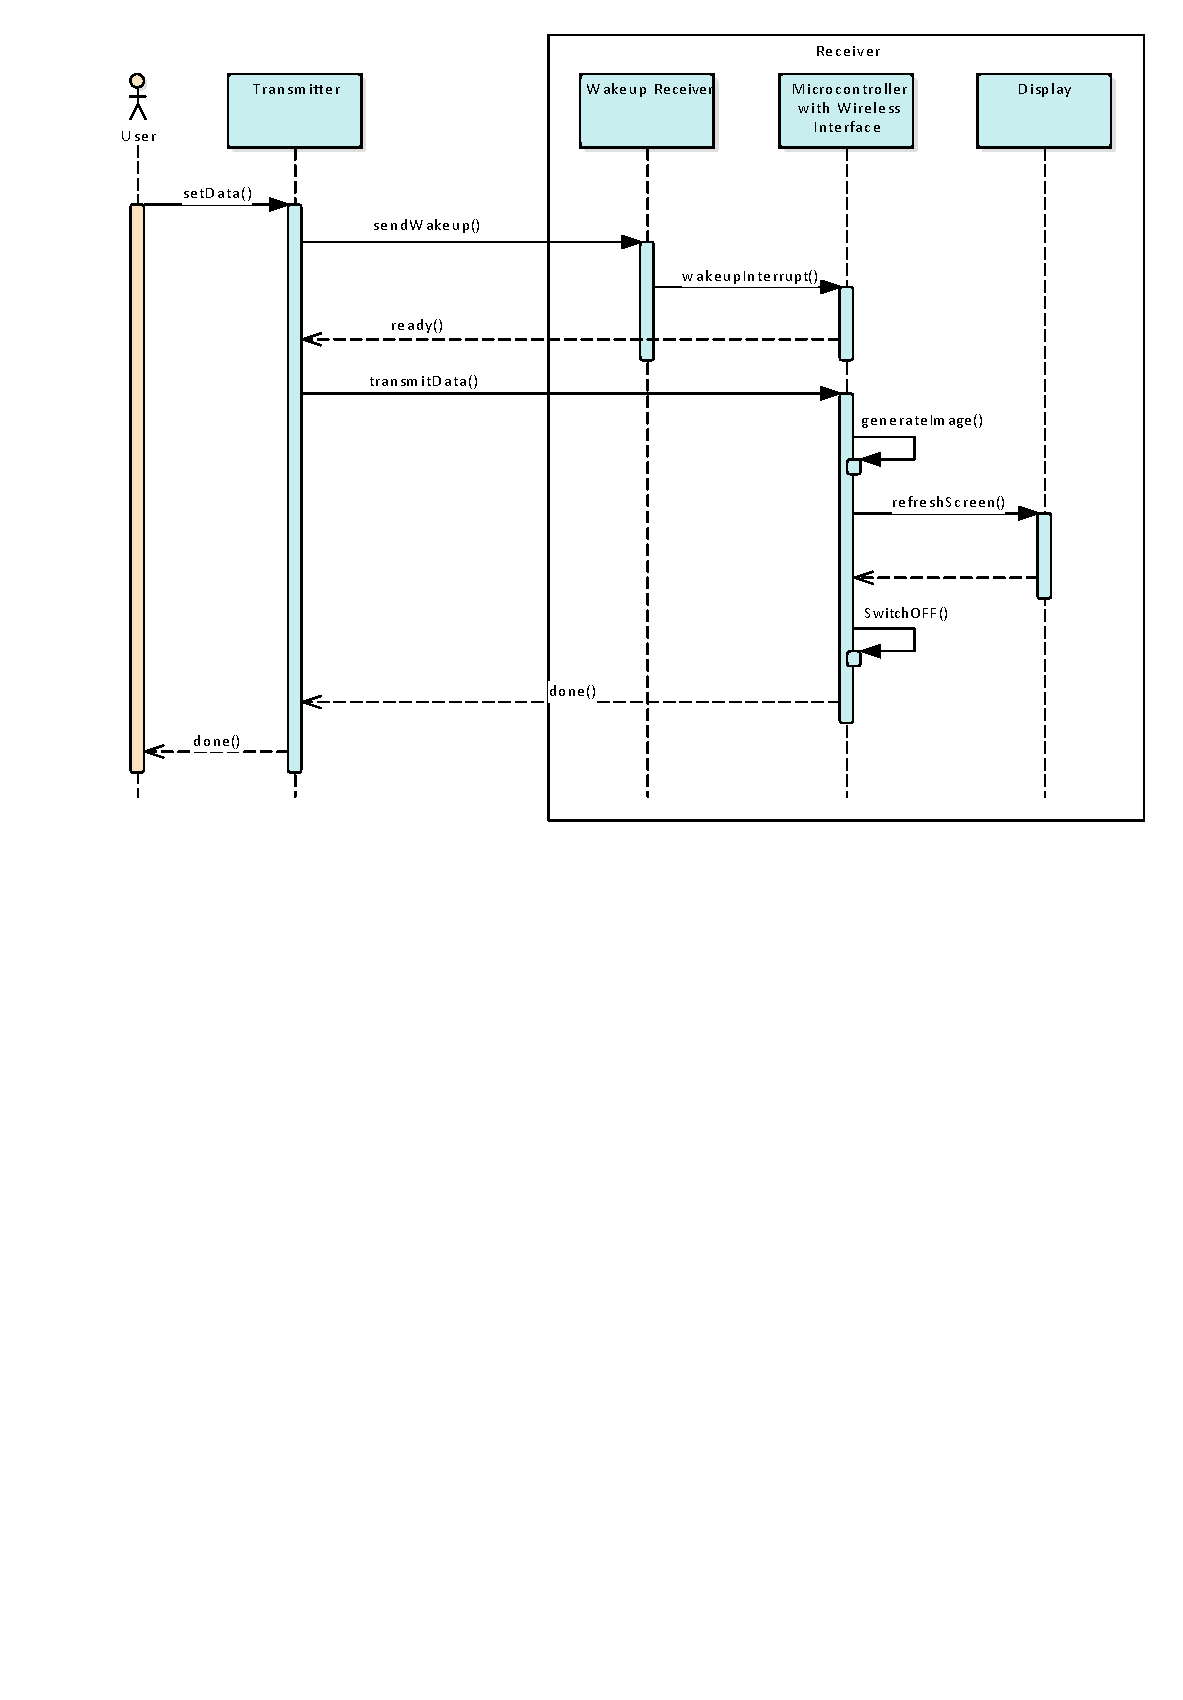
\includegraphics[width=0.9\textwidth]{4-development/software/graphics/sequence.pdf}
	\caption{not up to date sequence\label{software:sequence}}
\end{figure}


\subsection{Receiver}


\subsubsection{Microcontroller}
The main controller of the receiver is the STM32. To develop firmware for the microcontroller the Hardware abstractions layer provided by STMicroelectronics is used. The firmware running on the STM32 is responsible for the following tasks:
\begin{itemize}[H]
	\item[-] Initialize the IT8951 display driver chip
	\item[-] Receive data via UART from the BLE module
	\item[-] Generating the displayed image data from a template
	\item[-] Writing received text strings to the EPD
	\item[-] Writing the image data to the display driver via SPI
	\item[-] Control the power supply of all the different components
\end{itemize}
\paragraph{Configurations}

\begin{center}
	\begin{tabular}{ |c|c|c|c|c| } 
		\hline
		Description & Function &Pin number & Speed& Properties \\
		\hline
		\multirow{4}{4em}{SPI} 	& Chip select & PA0& &No Pull-up/-down \\ 
								& Clock& PA1 & 14.0 MBits/s&No Pull-up/-down \\ 
								& MISO & PA6&14.0 MBits/s & No Pull-up/-down  \\ 
								& MOSI & PA7& 14.0 MBits/s&No Pull-up/-down  \\ 
		\hline
		\multirow{2}{4em}{UART} & TX & PC10 & 115.2 kBits/s & Pull-up   \\ 
								& RX & PC11 & 115.2 kBits/s & Pull-up \\ 
	\hline
	\end{tabular}
\end{center}
\begin{figure}[H]
	\centering
	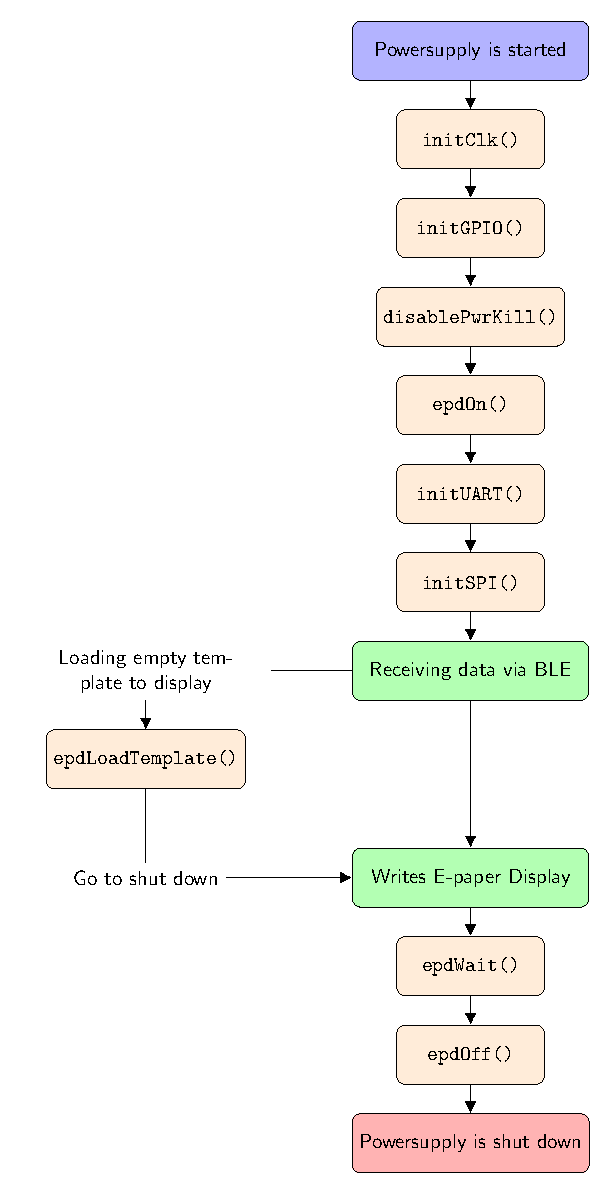
\includegraphics[height=0.8\textheight]{4-development/software/graphics/main.pdf}
	\caption{STM32 program flow chart\label{software:main}}
\end{figure}
In the flowchart\ref{software:main} it is visible that the controller itself never enters a deep sleep mode in the end of an program cycle. Instead the controller runs trough a power kill sequence which disables the own power supply. As a result of this the controller and remaining hardware consume no power instead of their deep sleep power consumption. 

\paragraph{Template}
The calendar template is getting preloaded in the flash of the STM32. To save memory, the file is converted into an $1200 \times 825$ PNG with the colour depth of 4 bit. The PNG then is used to create a .c file which holds an one dimensional array with all the pixel data in it.

\paragraph{Writing characters}
\lstdefinestyle{mystyle}{
	language=c,
	tabsize=4,
	showstringspaces=false,
	backgroundcolor = \color{gray!15!white},
	basicstyle=\scriptsize\ttfamily,
	morekeywords={as},
	keywordstyle=\color{red!80!black},
	stringstyle=\color{green!50!black},
	numberstyle=\color{red},
	emph={int,char,double,float, uint8_t, uint16_t},
	emphstyle=\color{green!50!black}
}
\lstset{style=mystyle}

\begin{figure}[ht!]
	\begin{lstlisting}
void drawChar(uint16_t Xpt, uint16_t Ypt, const char Acsii_Char,
					sFONT* Font, uint8_t cBackground, uint8_t cForeground)
	{
		uint16_t Page, Column;
		if (Xpt > Paint.Width || Ypt > Paint.Height) 
		{
			return;
		}
	uint32_t Char_Offset = (Acsii_Char - ' ') * Font->Height * 
							(Font->Width / 8 + (Font->Width % 8 ? 1 : 0));
	const unsigned char *ptr = &Font->table[Char_Offset];
	
	for (Page = 0; Page < Font->Height; Page ++ ) 
	{
		for (Column = 0; Column < Font->Width; Column ++ ) 
		{
			if (FONT_BACKGROUND == cBackground) 
			{ 
				if (*ptr & (0x80 >> (Column % 8)))
					Paint_SetPixel(Xpt+Column, Ypt+Page, cForeground);
			} 
			else 
			{
				if (*ptr & (0x80 >> (Column%8))) 
				{
					Paint_SetPixel(Xpt + Column, Ypt + Page, cForeground);					
				} 
				else 
				{
					Paint_SetPixel(Xpt + Column, Ypt + Page, cBackground);
				}
			}
			//One pixel is 8 bits
			if (Column % 8 == 7)
				ptr++;
		}
		if (Font->Width % 8 != 0)
			ptr++;
	}
}
	\end{lstlisting}
\end{figure}
\begin{figure}[ht!]
\begin{lstlisting}
void drawString(uint16_t xStart, uint16_t yStart,const char * pString, sFONT* Font,
							 uint8_t cBackground,uint8_t cForeground) 
{
	uint16_t Ypt = yStart;
	uint16_t Xpt = xStart;
	
	if (xStart > Paint.Width || yStart > Paint.Height)
	{
		return;
	}
	while (* pString != '\0') 
	{
		if ((Xpt + Font->Width ) > Paint.Width ) 
		{
			Xpt = xStart;
			Ypt += Font->Height;
		}
		if ((Ypt  + Font->Height ) > Paint.Height ) 
		{
			Xpt = xStart;
			Ypt = yStart;
		}
		Paint_DrawChar(Xpt, Ypt, * pString, Font, cBackground, cForeground);
		pString ++;
		Xpt += Font->Width;
	}
}	
\end{lstlisting}
\end{figure}


\subsubsection{Communication}
The software on both sides of the bluetooth channel is very similar, thus it is explained in this section.
A \acs{ble} example project, which was provided by nordic, was only slightly changed to fit the purpose of this prototype.

Before a connection is established, the module on the receiver side is known as peripheral, and the module on transmitter end as the central device.
After the receiver is woken up with the RFicient, the peripheral starts advertising.
Advertising basically means sending data packets periodically with information for the central device.
The central is scanning for the this advertisement and can based on this information decide, if it wants to connect.
Is the connection established, it is now possible to exchange data through this channel.
This process is illustrated in Figure \ref{software:ble}.
\begin{figure}[ht]
	\centering
	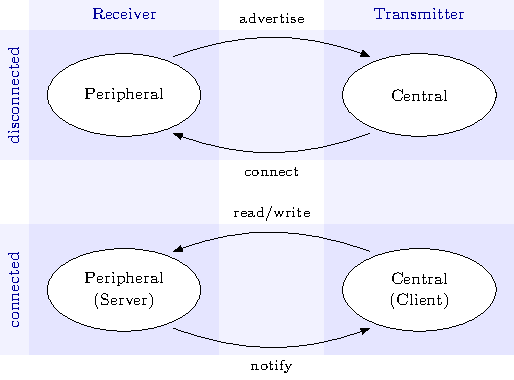
\includegraphics[width=0.8\textwidth]{4-development/software/graphics/ble.pdf}
	\caption{\acs{ble}-communication with the nRF52480.\label{software:ble}}
\end{figure}

The central serves after connection as the client.
It can make read and write requests to access the data on the peripheral, which acts as the server.
The server on the other hand can only send notifications to the client if new data is ready.
It should be noted, that the roles of client and server do not in any case have to be assigned to central and peripheral, but also the other way around. 

\subsection{Transmitter}

\subsubsection{Python-Script}
\lstset{basicstyle=\footnotesize}
\lstdefinestyle{mystyle}{
	language=Python,
	tabsize=4,
	showstringspaces=false,
	backgroundcolor = \color{gray!15!white},
	basicstyle=\scriptsize\ttfamily,
	morekeywords={as},
	keywordstyle=\color{blue!50!black},
	stringstyle=\color{green!50!black},
	numberstyle=\color{red},
	emph={int,char,double,float,range, len, bytes},
	emphstyle=\color{violet}
}
\lstset{style=mystyle}

A short python script enables the user to send the data to the display.
This script is looked at here step by step.

\begin{enumerate}
	\item Include of the used packages, time and serial.
	\begin{lstlisting}
	import serial
	import time
	\end{lstlisting}	
	\item Set desired baudrate, select which COM-port windows assigned to the development kit and open the port.
	\begin{lstlisting}
	baudrate = 115200
	com_port = 'COM14'
	
	device = serial.Serial(com_port, baudrate, writeTimeout=0)
	\end{lstlisting}
	\item Create a list of list with the desired data.
	The first list contains information about how many packages are about to follow.
	The following list contain the location on the template, the subject and the lecturer.
	\begin{lstlisting}
	data = [[0, chr(3), '\0\0\0\0'],[11 , 'WsComm\0', 'MAH\0'],
			[3 , 'DigPro\0', 'SCU\0'], [22 , 'EmbSW\0', 'BON\0']]
	\end{lstlisting}
	\item Fill the list with \lstinline|'\0'| so every package is 20 bytes long.
	\begin{lstlisting}
	for i in range(len(data)):
		if len(data[i][1])<16:
			t = 14-len(data[i][1])
			data[i][1] = data[i][1]+'\0'*t
	\end{lstlisting}
	\item Store time when data transfer is started.
	\begin{lstlisting}
	t_start = time.time()
	\end{lstlisting}
	\item Transfer data to the nRF52480 transmitter
	\begin{lstlisting}
	for i in range(len(data)):
		device.write([data[i][0]]) 
		device.write(bytes(data[i][1], 'utf-8'))       
		device.write(bytes(data[i][2]+'\n', 'utf-8'))
		device.flush()
	\end{lstlisting}	
	\item Print elapsed time on console and close COM-port.
	\begin{lstlisting}
	print('elapsed time: {:.3f}'.format(time.time() - t_start))
	
	device.close()
	\end{lstlisting}
	
\end{enumerate}